\documentclass[a4paper,oneside,11pt]{book} 
\usepackage[spanish]{babel} 
\usepackage[utf8]{inputenc} 
\selectlanguage{spanish}
\usepackage{latexsym} 
\usepackage{endnotes}
\usepackage{graphicx}
\usepackage{lscape}
\usepackage[T1]{}
\usepackage[pdftex=true,colorlinks=true,linkcolor = black,plainpages=false]{hyperref} % Soporte hipertexto
\oddsidemargin = 0.4 cm
\textwidth = 15.6 cm
\textheight= 22.5 cm
\topmargin = - 0.04 cm
\usepackage{lscape}

\usepackage{fullpage}
\usepackage{booktabs}
\usepackage{multirow}
\usepackage{wrapfig}
\usepackage{subfigure}
\usepackage{xcolor}
\usepackage{apacite}
\usepackage{fancyhdr} 
\usepackage{vmargin}
\usepackage{lipsum}
\pagestyle{fancy}
\usepackage{enumerate}
\usepackage{hyperref}



%\lhead{\begin{picture}(0,0){\includegraphics[width=1.2cm]{logo1.png}}\end{picture}}	
%\lhead{ \vspace{-0.1cm} \large{MANUAL PARA LA DIGITACIÓN DE BITÁCORAS DE PESCA}
%\vspace{0.1cm}}
%\rhead[\rchead{}]{}


\fancyhead[L]{\small MANUAL PARA LA DIGITACIÓN DE BITÁCORAS DE PESCA}
\fancyhead[C]{}
\fancyhead[R]{}
\fancyfoot[L]{Dirección General de Investigaciones de Recursos Pelágicos}
\fancyfoot[C]{}
\fancyfoot[R]{\thepage}
\renewcommand{\headrulewidth}{0.2pt}
\renewcommand{\footrulewidth}{0.2pt}
\usepackage{amsmath,amssymb,amsfonts}
\usepackage{color}
\definecolor{SolutionColor}{gray}{0.85}


\begin{document}

\begin{titlepage}


\begin{figure}
\centering

\includegraphics[width=8cm]{imagen_Manual_PBP/logo.png}
\end{figure}


\begin{center}
%\Large \textbf{IMARPE}\\
\vspace*{0.1in}
\large {DIRECCIÓN GENERAL DE INVESTIGACIONES DE RECURSOS PELÁGICOS} \\ 

\end{center}

\vspace*{0.6in}
\begin{large}
\end{large}
\vspace*{0.2in}
\begin{Large}
\begin{center}
\rule{150mm}{0.3mm}\\
\huge {\textbf{MANUAL PARA LA DIGITACIÓN DE BITÁCORAS DE PESCA}} \\
\rule{150mm}{0.3mm}\\
\end{center}
\end{Large}
\vspace*{0.1in}
\begin{large}
\end{large}
\vspace{60pt}

\noindent
\small{Usca C. Luis y Calderon M. Karla. En colaboración de: Ochoa M. Manuel, Alvis H. Lourdes, Chavez C. Rosa, Ticona P. Elizabeth, Piña G. Jorge, Vásquez G. Adriana, Salina R. Juan, Seminario P. Joselyn, Cancho C. Sandra.
Manual editado en el marco del proyecto “Estimación de Parámetros Biológico-Pesqueros para el manejo sostenible de los recursos marinos”.}\\
\vspace{10pt}
\begin{center}
\vspace*{0.1in}
\vspace*{0.1in}

\begin{large}
\Large {\textbf{Instituto del Mar del Perú} \vspace{5pt}\\ Callao - 2015}
\end{large}
\end{center}
\end{titlepage}


 
\newcommand{\figura}[4]{
  \begin{figure} 
  \begin{center} 
  \includegraphics[#2]{#1} 
  \caption{#3} 
  \label{#4} 
  \end{center} 
  \end{figure}} 

\newenvironment{tabla}[2]{ 
  \begin{table} 
  \begin{center} 
  \caption{#1} 
  \label{#2}}{\end{center} 
  \end{table}} 




\renewcommand{\contentsname}{CONTENIDO} 
\renewcommand{\partname}{Parte} 
\renewcommand{\chaptername}{Capítulo} 
\renewcommand{\appendixname}{Apéndice} 
\renewcommand{\bibname}{Bibliografía} 
\renewcommand{\figurename}{Figura} 
\renewcommand{\listfigurename}{Índice de figuras} 
\renewcommand{\tablename}{Tabla} 
\renewcommand{\listtablename}{Índice de tablas}  


\tableofcontents 

\chapter {INTRODUCCIÓN}

EL PROGRAMA BITÁCORAS DE PESCA (PBP) fue implementado por el IMARPE en 1996 como un programa de observadores a bordo de la flota industrial pelágica con el objetivo primario de colectar información sobre medidas de esfuerzo efectivo para la estimación de índices de abundancia relativa de la anchoveta (Bouchon et al. 1998).
Con el transcurrir del tiempo, nuevos objetivos se fueron añadiendo hasta convertir al programa en un medio capaz de monitorear los movimientos de la flota, los descartes, la captura incidental, el comportamiento de los recursos, su distribución y estructura demográfica, la interacción con los depredadores superiores e incluso el ambiente.\\

Actualmente el programa forma parte del objetivo de investigación EVALUACIÓN INDIRECTA DE LOS PRINCIPALES RECURSOS PESQUEROS y esta a cargo de la Unidad de Investigaciones en Dinámica Poblacional (UIDINP) de la Dirección de Investigaciones de Recursos Pelágicos - Neríticos y Oceánicos (DIRPNO).\\

Como parte del  proyecto “Estimación de Parámetros Biológico-Pesqueros para el manejo sostenible de los recursos marinos”, se ha iniciado el ingreso y validación de la información de las bitacoras de pesca al sistema de almacenamiento de datos IMARSIS, desde los años 1996 hasta la actualiddad y como una guía para el ingreso de datos, se ha elaborado el presente manual, con el objetivo de velar por la calidad de información que se cuente para un análisis adecuado de los mismos.

\newpage
\section{Objetivo general del proyecto}

\begin{enumerate}
\item Realizar estudios permanentes de diferentes medidas de esfuerzo pesquero que permitan una adecuada estimación de la abundancia relativa de los principales recursos pelágicos.
\item Determinar las variaciones espacio-temporales de los componentes biológicos de los principales recursos pelágicos (densidad, tallas, profundidad, entre otros).
\item Aportar al entendimiento de la dinámica de la flota de cerco (inversión/reinversión, asignación de esfuerzo pesquero, rendimientos, descartes).
\end{enumerate}

\section{Objetivos del manual}

 \begin{enumerate}
 \item Describir los procedimientos de manera detallada y clara, para la correcta digitación de los datos.
  \item Brindar al profesional encargado en el ingreso de datos las herramientas necesarias como los conocimientos y criterios a considerar durante el ingreso de información de cada ficha.
 \end{enumerate}
 

\section{Sobre profesional para el ingreso de datos}
El $"$digitador$"$ es considerado un  profesional de la carrera de Ing. Pesquera y/o Ciencias Biológicas con conocimiento en pesquería, cuyas funciones dentro del trabajo son:
\begin{itemize}
\item Ingresar la información biológico-pesquero, embarcación, plantas de desembarque, etc. de las bitacoras de pesca al sistema IMARSIS, considerando la importancia de esta para su posterior análisis y aplicación.
\item Verificar la veracidad de la información almacenada en fichas y/o libros bitacoras.
\item Consultar datos incongruentes o faltantes y nunca inferir información al momento de registrar en el IMARSIS.
\item Identificar adecuadamente los datos con mucha atención, ya que existe información parecida que conlleva al error en el registro.\\
\end{itemize}



\chapter{INFORMACIÓN GENERAL BITÁCORAS}

\section{Bitacoreros}

Actualmente el programa cuenta con 20 observadores, entre Biólogos, Ingenieros y Tecnólogos Pesqueros, estratégicamente localizados en los principales puertos de desembarque de recursos pelágicos a lo largo de todo el litoral peruano.
Dicho personal se instala de manera aleatoria, a bordo de embarcaciones de la flota industrial de cerco y colecta la información  biológica-pesquera resultante de las actividades que realizan dichas embarcaciones durante un viaje de pesca.
La información es anotada en las denominadas BITÁCORAS DE PESCA las mismas que son centralizadas por la UIDINP. La información contenida en ellas es digitada y almacenada en una base de datos para su posterior procesamiento y análisis.


\section{De la embarcación} 
Una Bitácora de Pesca es un formulario que consta básicamente de dos partes:\\
La primera donde se describe, mediante el uso de una simbología establecida, todas las actividades que realiza una embarcación desde el momento del zarpe hasta el arribo, planta o fabrica de desembarque, datos de captura (Captura total, envasada, ofrecida, descarte, desb. estimado, recibida, capt. oficial). En estas fichas se consigna además información sobre la embarcación (tamaño, material y equipamiento) y la tripulación (número, edad promedio), tipo de arte utilizado, tipo de viaje, etc.

 \begin{figure}[!h]
  \begin{center} 
 \fbox{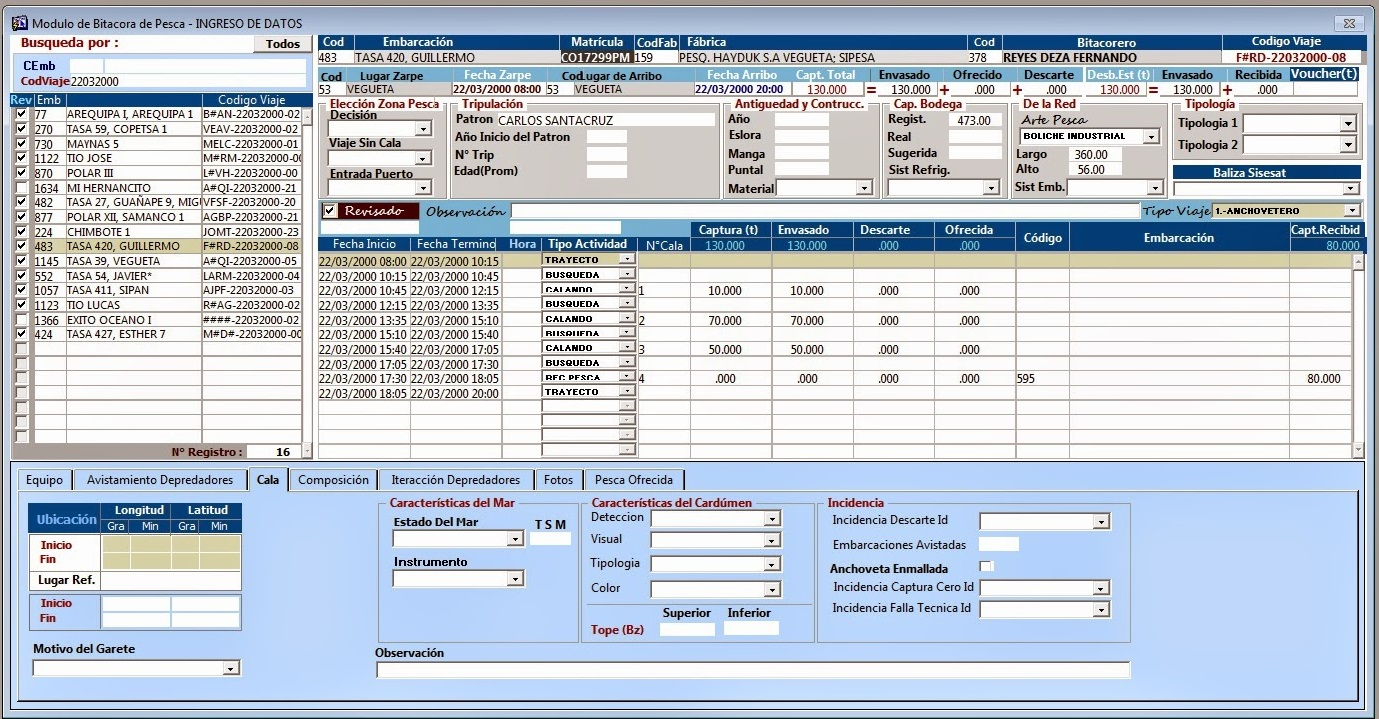
\includegraphics[scale=0.4]{imagen_Manual_PBP/imar.jpg}}
  \caption{Interfas del IMARSIS.}
 \end{center}
  \end{figure}

En la segunda, que es elaborada para cada lance u operación de pesca, se ahonda en la información biológica como la biometría, composición por especies de la captura, hora, profundidad del cardumen, avistamiento de depredadores superiores, entre otros.
A partir de toda la información colectada por viaje, las variables obtenidas pueden ser asociadas en tres grupos:

\section{Del viaje} 
Con registrar tan sólo el nombre y la matrícula de la
embarcación y a partir del cruce de estas variables con bases de datos de las características de la flota, se pueden deducir muchas otras. Estas son la capacidad de bodega, TRB, material, año de construcción, medidas, sistema de refrigeración, permisos de pesca, tipos y tamaños de redes, etc.

\section{Del lance}
 \begin{figure}[!h]
  \begin{center} 
 \fbox{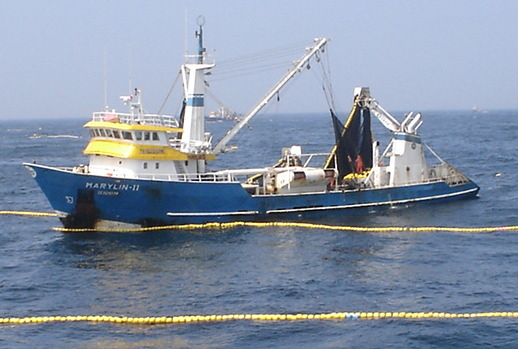
\includegraphics[scale=0.6]{imagen_Manual_PBP/0123}}
  \caption{Boliche industrial.}
 \end{center}
  \end{figure}

A cada lance efectuado durante el viaje le correspondería la hora, posición exacta, duración, captura, composición por especies, profundidad, horas de búsqueda previa y tallas para cada especie capturada.

Puertos de salida y llegada, hora de salida y llegada, duración,
horas empleadas en la búsqueda de cardúmenes, número de lances
efectuados, captura total.


\chapter{BITÁCORAS DE PESCA} 
Esta sección permite que el usuario logre conocer los comandos necesarios para el ingreso y al acceso de información científica al IMARSIS. Antes de iniciar con la digitación de datos provenientes de las fichas, es necesario verificar la instalación correcta del IMARSIS PELÁGICO, que será visualizada a través de un ícono con acceso directo, visulizado en escritorio, así mismo se deberá verificar la instalación correcta del internet, ya que el sistema trabaja con conexión directa, de lo contrario no se podrá guardar ningun ingreso de información.
Si persistieran problemas con el usuario, conexión de internet o  con el sistema IMARSIS, comunicarse directamente con el Área Funcional de Informática. 

\section {Pasos para acceder al sistema IMARSIS}

\begin{itemize}
\item\textbf{Paso 1:}\\
Dirigirse al ícono \textbf{BITÁCORA 2014 PRODUCCIÓN} ubicado en el escritorio y hacer doble click.
\item\textbf{PASO 2:} \\
Una vez abierto el ícono \textbf{BITÁCORA 2014 PRODUCCIÓN}, aparecerá una ventana con el acceso al sistema \textbf{IMARSIS}, en el cual se tendrá que seleccionar el nombre del usuario, según:\\
\subitem\textbf{Usuario:} Nombre y apellido del digitador.
\subitem\textbf{Contraseña:} DNI del usuario, será visualizado en modo clave.
\begin{figure}[htbp]
\centering
\subfigure[Ícono del IMARSIS]{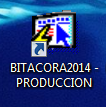
\includegraphics[width=40mm]{imagen_Manual_PBP/BITACORA2014}}
\subfigure[Login]{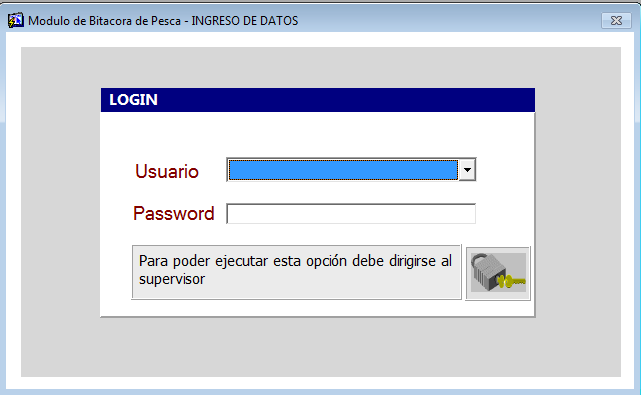
\includegraphics[width=60mm]{imagen_Manual_PBP/login}}
\caption{Acceso al sistema bitácoras.}
\vspace{-10pt}
\end{figure}

\item\textbf{PASO 3:}\\
Luego de haber ingresado al sistema de \textbf{BITÁCORA 2014 PRODUCCIÓN}, aparecerán las casillas activas vacías.
 \begin{figure}[!h]
  \begin{center} 
 \fbox{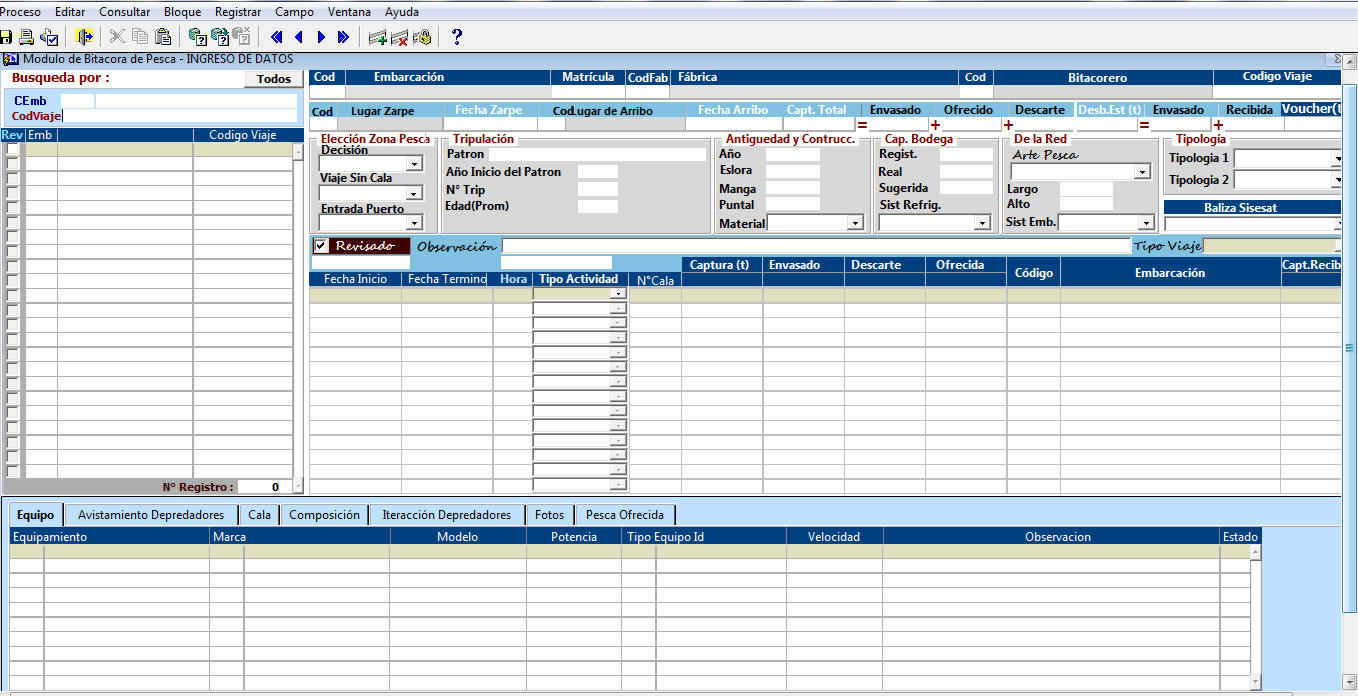
\includegraphics[scale=0.4]{imagen_Manual_PBP/blanco}}
  \caption{Plantilla de bitácoras.}
 \end{center}
  \end{figure}

 \end{itemize}
  
\section {Partes de una ficha bitácora}
\subsection{Íconos del sistema}
  \begin{figure} [!h]
  	\begin{center}
  		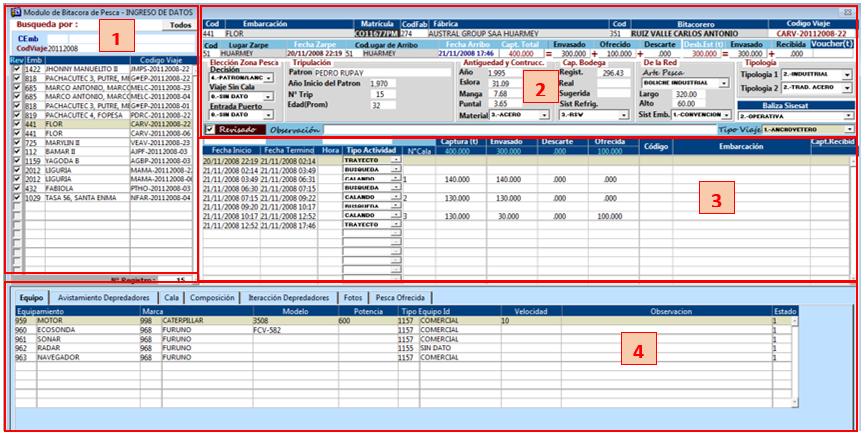
\includegraphics[scale=0.6]{imagen_Manual_PBP/seccion.png}
  		\caption{División de una ficha bitacora.}
  	\end{center}
  \end{figure}


\begin{itemize}
\item {Antes de insertar una ficha es necesario conocer la función de los comando del margen superior, en especial tener en cuenta el ícono necesario para crear un nuevo registro y para salir del sistema.}
\item {Es importante que si se dejara de digitar por un largo tiempo, mayor a 10 minutos, se recomienda guardar los cambios y cerrar la sesión,ya que el tener demasiado tiempo abierto el programa, sin ingresar un dato, podrá perder toda la información ya digitada.}
\end{itemize}
  \begin{figure} [!h]
  	\begin{center}
  		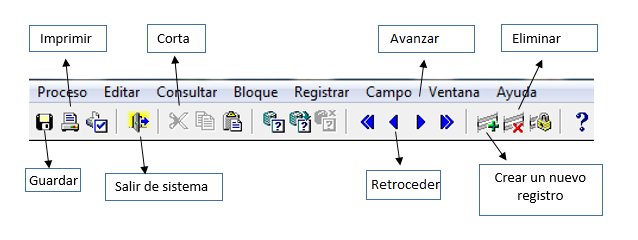
\includegraphics[scale=0.85]{imagen_Manual_PBP/casillas.png}
  		\vspace{-20pt}
  		\caption{Íconos del encabezado.}
  	\end{center}
  \end{figure}
 
 \subsection{División del interfas en el IMARSIS}
 \begin{enumerate}
 \item Sección referente a la búsqueda
 \item Sección sobre captura total y embarcación
 \item Sección sobre el lance
 \item Sección sobre equipos e información de composición por cala
 
 \end{enumerate}
 
\section{Descripción primera sección }
\subsection{Búsqueda de viajes}

En esta sección existe dos formas de buscar un viaje, bien por código de embarcación (CEmb) o el código de viaje (CodViaje) como por ejemplo CARV-20112008-22 que corresponde a la embarcación
Flor con las inicales del bitacorero CARV que corresponde a Ruiz Valle Carlos Antonio. En el caso que  la ficha no indique el bitacorero, aparecerá como BTNF (Bitacorero No Definido).
En algunas ocasiones las fichas ya están ingresadas, entonces el digitador lo que hace es revisar la veracidad de la información, corrigiendo algunos errores, en consecuencia, el viaje debería aparecer con el check correspondiente.
\begin{figure} [!h]
  	\begin{center}
  		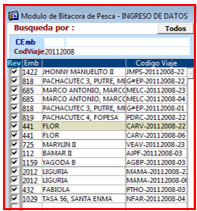
\includegraphics[scale=1]{imagen_Manual_PBP/codigo}
  		\vspace{-5pt}
  		\caption{Búsqueda por viaje.}
  	\end{center}
  \end{figure}


\section{Descripción segunda sección}

Esta sección es de vital importancia ya que forma parte del único registro que se genera de todo el viaje, y con ello, el código generado en el sistema. El incorrecto ingreso de esta información, invalida la búsqueda y la extracción de los datos.
 \begin{figure} [!h]
 	\begin{center}
 		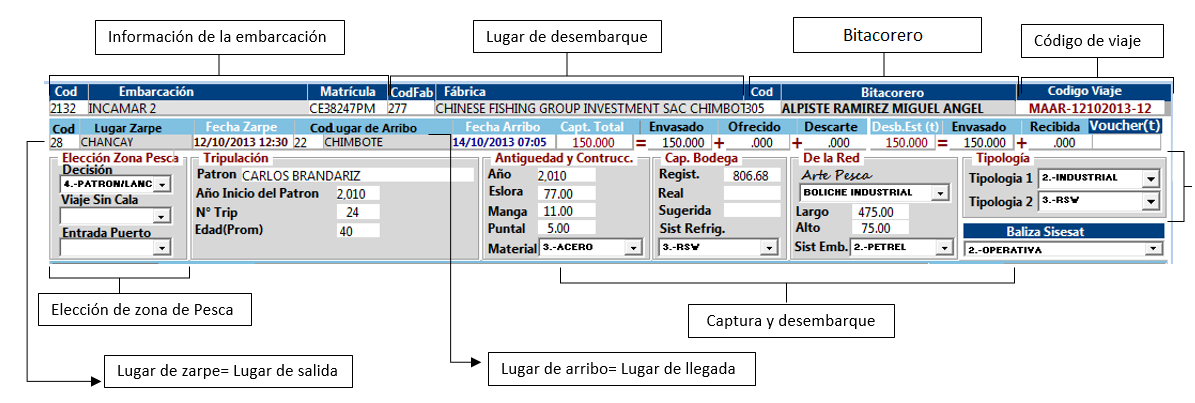
\includegraphics[scale=0.47]{imagen_Manual_PBP/partes.png}
 		\caption{Partes de la segunda sección.}
 	\end{center}
 \end{figure}

 
 \begin{enumerate}
 \item\textbf{ Embarcación:} esta casilla permite realizar la búsqueda de la embarcación; al ubicarse en la casilla, con un doble click o bien presionando la tecla \textbf{F1}.
 
 \item [] \textbf{$\ast$ Importante}: muchas embarcaciones tienen varios nombres o seudonimos, hayan realizado cambios o no esten registrados todavía en el sistema; en estos casos, agotar todos los modos posibles de búsqueda, consultando según su matrícula en la página web del PRODUCE, en la sección de embarcaciones pesqueras \url{http://www.produce.gob.pe/index.php/servicios-en-linea/embarcaciones-pesquera} y por último colsultar al analista encargado.
 Si hasta la fecha la embarcación, sea el caso de que haya cambiado de nombre, que posiblemente el sistema lo registre con dos nombres como:   \\ Don Nicola, Bibaco 23 , el sistema no lo encontrará, ya que Bibaco 23 está con el segundo nombre de Don Nicola.\\
\item [] Para que el sistema encuentre a \textbf{Bibaco 23}, deberá hacerse una búsqueda colocando el nombre entre porcentajes, ejemplo :
 \textbf{ \% Bibanco 23 \%}
 
 \begin{figure}[htbp]
 	\centering
 	\subfigure[Búsqueda]{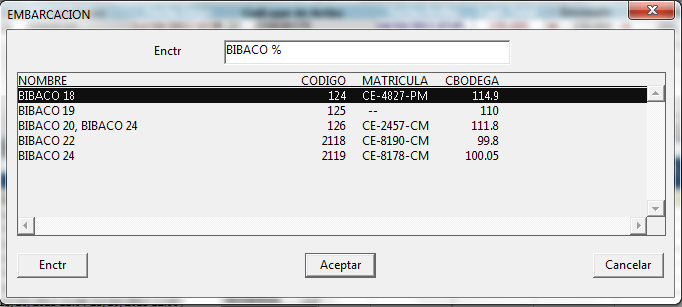
\includegraphics[width=70mm]{imagen_Manual_PBP/bibaco}}
 	\subfigure[Búsqueda]{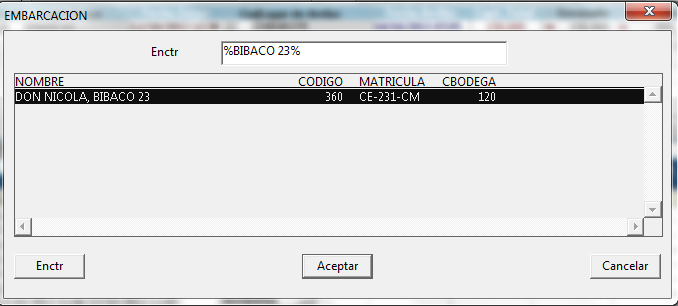
\includegraphics[width=70mm]{imagen_Manual_PBP/bibaco3}}
  	\caption{Ejemplo de búsqueda.}
 	\vspace{-10pt}
 \end{figure}
 
 \item \textbf{Fábrica o planta de desembarque:} casilla también denominada en ficha, como lugar de desembarque, para seleccionar fábrica presionar \textbf{ F1}, se recomienda realizar la búsqueda entre porcentajes. Ejemplo:  \textbf{\% HAYDUK \%}.
 En los lugares de desembarque existen muchas plantas o fábricas, considerar lo que indica en la ficha y si no estuviera  registrado la planta en el IMARSIS, reportar al analista encargado para que agregue en el sistema.
  
 \item[] Solo así, colocando en porcentaje la búsqueda tendremos la seguridad que podemos extraer todos los datos que coincidan con \textbf{HAYDUK.}
  \begin{figure} [!h]
  	\begin{center}
  		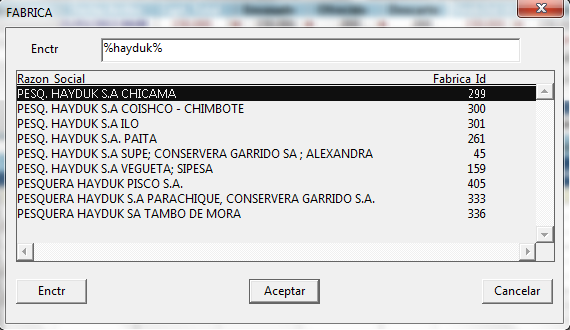
\includegraphics[scale=0.7]{imagen_Manual_PBP/hayduk.png}
  		\caption{Herramientas a utilizar en la búsqueda de embarcación.}
  	\end{center}
  \end{figure}
  \begin{figure} [!h]
  	\begin{center}
  		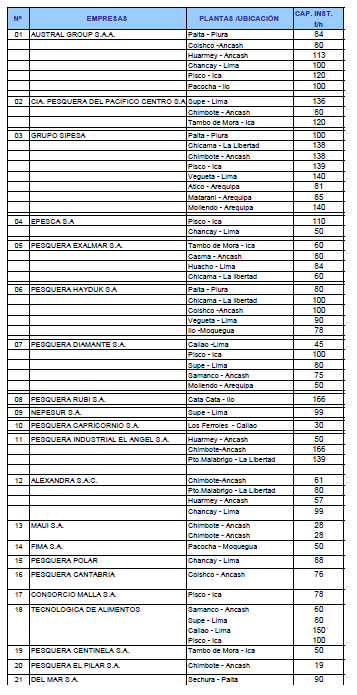
\includegraphics[scale=1]{imagen_Manual_PBP/planta1}
  		\caption{Empresa pesquera y planta de desembarque.}
  	\end{center}
  \end{figure}
  
  \begin{figure} [!h]
   	\begin{center}
   		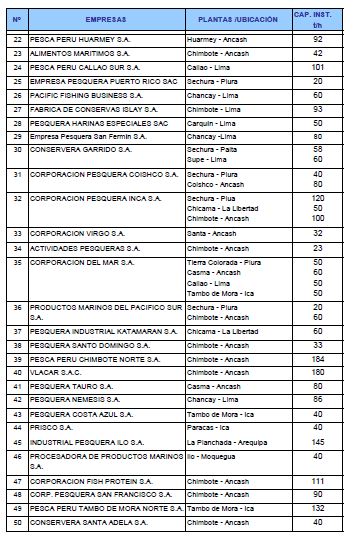
\includegraphics[scale=1]{imagen_Manual_PBP/planta2}
   		\caption{Empresa pesquera y planta de desembarque}
   	\end{center}
  \end{figure}
\item \textbf{{Bitacorero:}} es la persona responsable de la toma de datos en ficha, cuyas iniciales del nombre del bitacorero, generarán las primeras iniciales del código de viaje. Se en contrará muchas fichas sin registro de bitacorero, lo cual se ingresará como no definido y si no estuviera en el sistema, pedir que se agregue. En ocasiones existen vieajes que coenciden en la hora de salida, lo cual no les permitirá ingresar ambos como no definido, esto se resuelve ingresando el segundo viaje con el nombre del usuario (digitador).

\item \textbf{{Lugar de zarpe y arribo:}} son los lugares donde inicia y acaba un  viaje con sus respectivas fechas y horas. Ojo que las fechas y horas deben coincidir con la actividad (trayectos) del viaje de la sección Nro 3.

\item \textbf{{Captura  total (t):}} en esta parte se registra la captura total que es la suma de lo envasado más lo ofrecido y el descarte (\textbf{Capt.Total (t)=Envasado + Ofrecido + Descarte}). Luego está el desembarque estimado que es la suma de lo envasado más lo recibbido (\textbf{Desb.Est(t)= Envasado + Recibido}). Finalmente está el \textbf{voucher(t}) que viene a ser la boleta de peso o boleta de pesaje de la captura oficial.

\item [] \textbf{$\ast$ Observación}: tener cuidado en esta parte, las capturas deben estar en una misma unidad (t) y a la vez  debe coencidir con las capturas totales por cala.

\item \textbf{{Elección zona de pesca:}}

\subitem{\textbf{Decisión}} indica quién determina la elección de la zona donde se va ha calar.
\subitem{\textbf{Viaje sin cala}} indica cuál fue el motivo que no hubo cala, si fue por mal tiempo, no hubo recurso, falla mecánica, etc.
\subitem{\textbf{Entrada a puerto:}} indica los motivos por los cuales se regresa a puerto, siendo las reparaciones u otros los determinantes.

\item \textbf{{Tripulación:} } información referente al patrón, año de inicio y número.

\item \textbf{{Antigüedad y construcción:}} corresponde a las características de la embarcación.

\item \textbf{{Capacidad de bodega:}} indica la capacidad de bodega de la embarcación, que sirve para determinar el tipo de pesquería. Si no presentara la información en la ficha, es recomendable consultar en la página wed del PRODUCE \url{http://www.produce.gob.pe/index.php/servicios-en-linea/embarcaciones-pesqueras} en la cual se encuentra toda la información respecto a las embarcaciones. Pudiendo buscar por nombre y/o matrícula, una vez identificado la embarcación, pinchar en busca y saldrá toda la información referente.
\begin{figure}
\centering
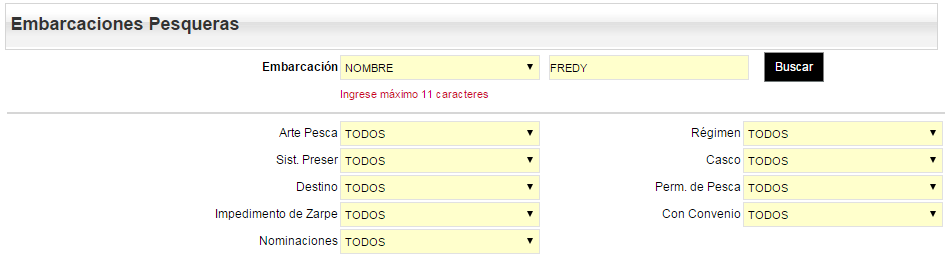
\includegraphics[width=0.7\linewidth]{./imagen_Manual_PBP/prod1}
\caption{Búsqueda por nombre o matrícula en PRODUCE}
\label{fig:prod1}
\end{figure}
\begin{figure}
\centering
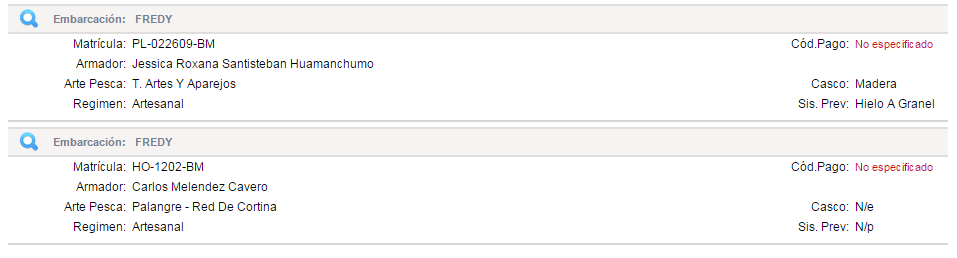
\includegraphics[width=0.7\linewidth]{./imagen_Manual_PBP/prod2}
\caption{Información de embarcación}
\label{fig:prod2}
\end{figure}

\item \textbf{{Datos de la red:}} en este item se va ha considerar la capacidad de bodega. Años anteriores al 2011 se consideraba en dos tipos de pesquerías: la artesanal que agrupaba a enbarcaciones con cap. bodega menores a 32.5t y las industriales con cap. bodega mayores a 32.5t, hecha esta observación, el tipo de red se colocará aquella que indique la ficha de bitacora. Genralmente las pesquerías anteriores a los años 2001 estaban dirigigas a la anchoveta (tamaño de malla 13mm) pudiendo capturar otras especies como caball/sard/jurel.

\item \textbf{{Tipología:}} indica los tipos de embarcaciones según capacidad de bodega (tipología 1) y si tienen sistema de enfriado RSW (topología 2). 

\end{enumerate}


\section{Descripción tercera sección } 
Corresponde al tipo de actividad realizada en cada viaje. Una vez acabada la segunda sección, se elige el tipo de viaje ya sea anchovetera, sard/jurel/caball, etc., luego se marca la casilla de revisado para poder continuar respecto a la actividad. Las capturas por cala debe ser la suma de lo envasado, descarte y ofrecido. El tipo de actividad se divide en:

\begin{itemize}
\item{\textbf{Trayecto}} 
Es la actividad realizada desde la salida de puerto hasta llegar al lugar o área de pesca.
\item{\textbf{Búsqueda}} 
Una vez llegado a la zona de pesca, se realiza la busqueda utilizando equipos de detección como la ecosonda, sonar,etc. hasta el momento de la cala.
\item {\textbf{Calando}} 
Conocido tambien como lance, es la actividad de captura del recurso.
\item{ \textbf{Garete}} 
Se considera una actividad dentro del viaje de pesca que significa fondear o quedarse en el mar por una actividad. Al registrar no olvidar el motivo de garete además de alguna información adicional como coordenadas, etc.

\item{\textbf{Rec pesca}} 
O pesca recibida de otra embarcación por diferentes motivos. Se tiene que ingresar el código de la embarcación que está regalando la pesca (ver fig. Nro 12). 

\end{itemize}
\begin{figure}
\centering
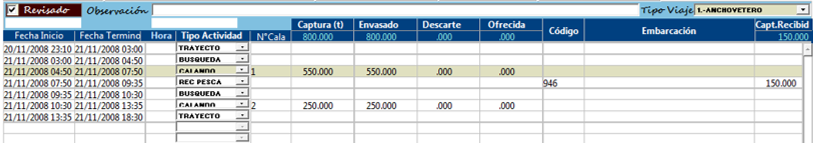
\includegraphics[width=1\linewidth]{./imagen_Manual_PBP/seccion3}
\caption{Tipo de actividad}
\label{fig:seccion3}
\end{figure}


\begin{itemize}
\item [] \textbf{$\ast$ Observación}: tener mucho cuidado al ingresar las fechas y horas de cada actividad, considerando toda la información existente para cada acto. Si no hubiera captura, entonces se llena con ceros cada casilla.
\end{itemize}

\section{Descripción cuarta sección } 
Esta sección requiere mayor esfuerzo de acuerdo a la cantidad de datos por ingresar. 
\subsection{Equipo} 
Respecto a la información de equipo, las fichas anteriores al año 2009 no cuentan con datos de equipo, como se explica más adelante. El equipamiento va detallado según el motor, ecosonda, sonar, radar, navegador, radio, etc. 
\begin{figure}
\centering
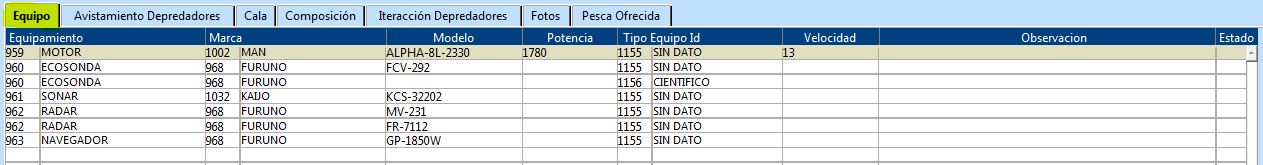
\includegraphics[width=1\linewidth]{./imagen_Manual_PBP/equipo}
\caption{Equipos utilizados por la embarcación}
\label{fig:equipo}
\end{figure}

\subsection{Avistamiento depredadores}

Se considera a la observación y registro de depredadores supereiores durante el trayecto de una embarcación más no en la cala, por lo general cetáceos. Se debe considerar minuciosamente toda los datos presente en la ficha bitácora, las distancias deben estar en km.

\begin{figure}
\centering
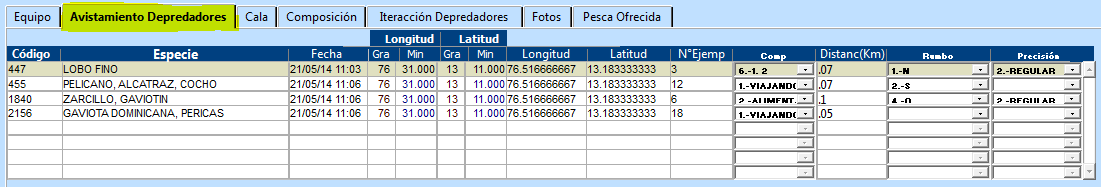
\includegraphics[width=1\linewidth]{./imagen_Manual_PBP/avista}
\caption{Ejemplo de registro avistamiento depredadores.}
\label{fig:avista}
\end{figure}

\subsection{Cala}
Cala o lance es el evento que se realiza cuando el recurso haya sido detectado para capturarlo, y es caracterizado por:
\begin{itemize}
\item{\textbf{Ubicación:}} 
coordenadas donde se realizo la cala (inicio y final) y el lugar de referencia.
\item{\textbf{Estado del mar:}} 
 va desde calmo hasta fuerte. También está el registro de la temperatura superficial del mar (TSM) y el tipo de instrumento utilizado.
\item{\textbf{Caracteristicas del cardumen:}} 
determina  cómo se observa el cardumen y con qué elementos, según:
\subitem \textbf{Detección:} 
modo de detección del cardumen, pudiendo ser: ecosonda, sonar, visual, o la combinación de estos.
 \begin{figure}[htbp]
 	\centering
 	\subfigure[Equipo detección]{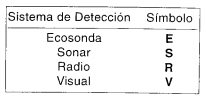
\includegraphics[width=30mm]{imagen_Manual_PBP/detec}}
 	\subfigure[Detección visual]{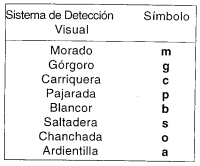
\includegraphics[width=50mm]{imagen_Manual_PBP/visual}}
 	\subfigure[Topes superior e inferior.]{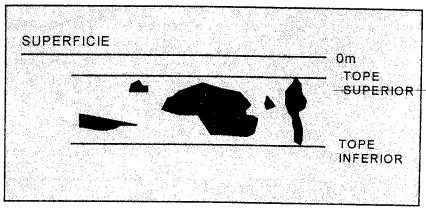
\includegraphics[width=50mm]{imagen_Manual_PBP/topes}}
  	\caption{Tipo de sistema de detección.}
  \end{figure}

\subitem \textbf{Visual:} cuando la embarcación utiliza como tipo de detección la visión, se emplea la terminología (ver fig.15).

\subitem \textbf{Tipología:} indica como está el recurso, pudiendo encontrarse en cardumen, estrato, mixto o disperso.

\subitem \textbf{Color:}  el color indica una forma estándar de abundancia del recurso. Por ejemplo el azul indica que el recurso está disperso o es sustrato, el verde,  pequeños sustratos  o algún acompañante, el amarillo, son manchas no tan densas y el  rojo, son manchas densas grandes y con formas en función a la especie.

\item{\textbf{Incidencia:}} indica el motivo de descarte, número de embarcaciones avistadas, anchoveta enmallada, motivo de captura cero y si hubo o no falla técnica.

\item{\textbf{Topes:}} es considerado la profundidad del cardumen momentos previo a la cala, considerándose el tope superior e inferior.

\end{itemize}

\begin{figure}
\centering
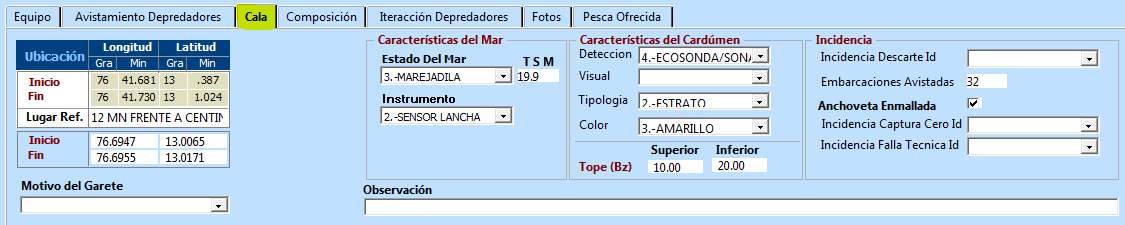
\includegraphics[width=0.95\linewidth]{./imagen_Manual_PBP/cala2}
\caption{Ejemplo datos cala}
\label{fig:cala2}
\end{figure}

\subsection{Composición}
Todas las especies capturadas en la cala (según la figura). Se registra los datos biométricos de las especies de la muestra, considerando sus tipos de medición. En las fichas bitácoras se ha registrado a las especies tanto con nombres científicos como los nombres comunes, para este último caso, se consulta con la bibliografía recomendada (Chirichigno,1998) para su correcto ingreso en el IMARSIS. 
\begin{figure}
\centering
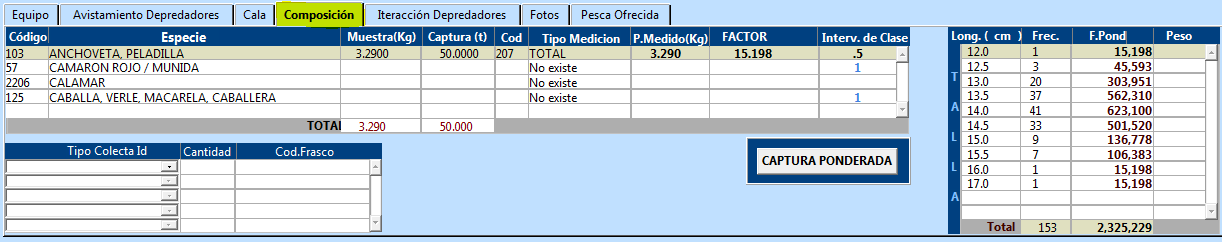
\includegraphics[width=1\linewidth]{./imagen_Manual_PBP/comp}
\caption{Tallas mínimas y tipo de medición recursos hidrobiológicos}
\label{fig:comp} 
\end{figure}
\begin{figure}[htbp]
 	\centering
 	\subfigure[Recursos marinos]{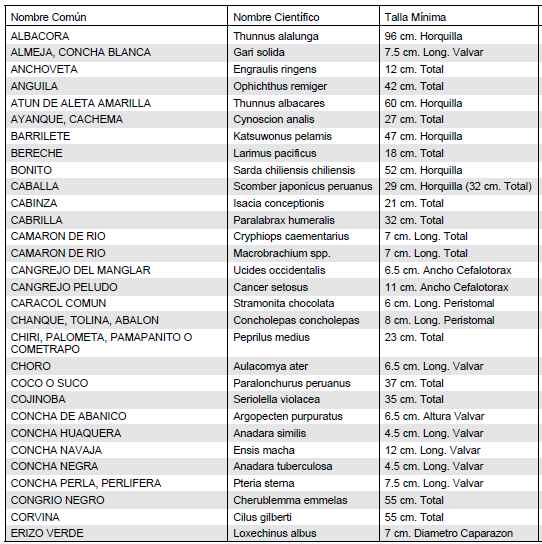
\includegraphics[width=70mm]{imagen_Manual_PBP/medi1}}
 	\subfigure[Recursos marinos]{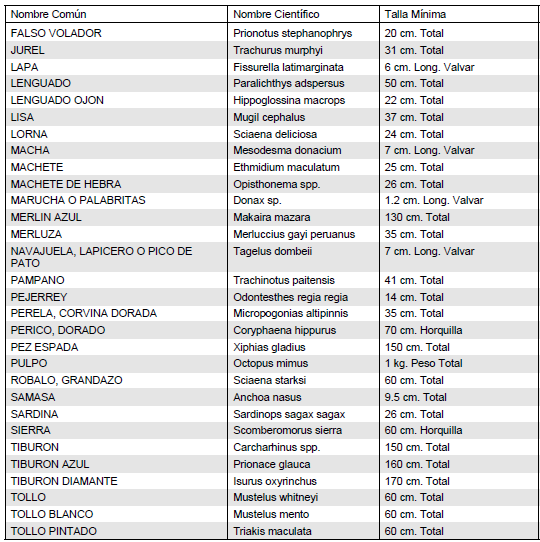
\includegraphics[width=70mm]{imagen_Manual_PBP/medi2}}
  	\caption{Tipo de medición recursos hidrobiológicos.}
 	\vspace{-20pt}
 \end{figure}
 
 \begin{figure}
\centering
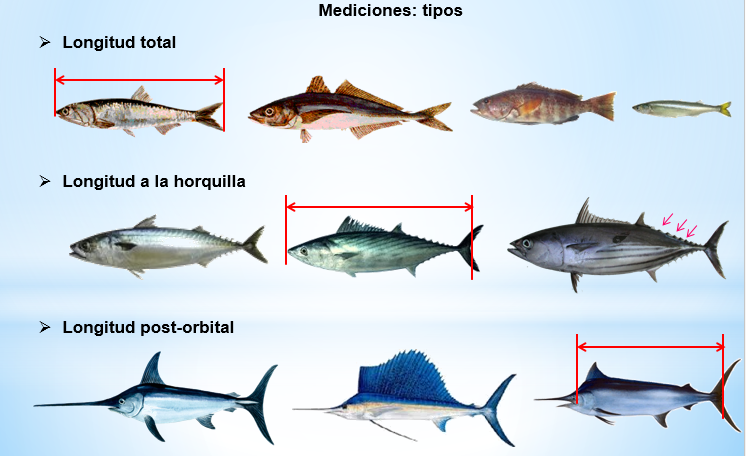
\includegraphics[width=0.7\linewidth]{./imagen_Manual_PBP/tipomedi}
\caption{Mediciones peces}
\label{fig:tipomedi}
\end{figure}


\subsection{Interacción depredadores}
Aquellas especies que están presente al momento de la cala, tales como los lobos marinos, las aves, algunos delfines. Se debe considerar la cantidad, en qué momento se ha observado,  el comportamiento, si hubo captura o no y en qué estado. Tambien se considera el grado de certeza, si hubo medición biométrica de aves y/o de tortugas.

\begin{figure}
\centering
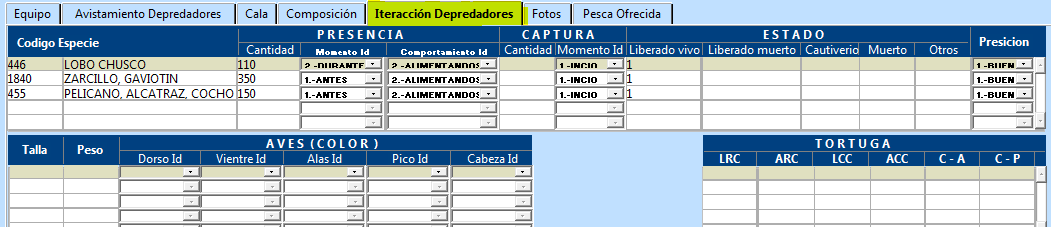
\includegraphics[width=1\linewidth]{./imagen_Manual_PBP/inter}
\caption{Ejemplo especies en interacción depredadores}
\label{fig:inter}
\end{figure}


\subsection{Fotos} Se registra la codificación de fotos tomadas.

\subsection{Pesca ofrecida} Es parte de la captura que se ofrece o traspasa a otra embarcación, siendo el exceso de capacidad de bodega la razón o no sea el recurso capturado el objetivo del patrón.\\

$\ast$ \textbf{Observación}: respecto a las especies que van a ser ingresadas en avistamiento, composición e interacción se tiene que hacer clara diferencia. Los peces e invertebrados tienen que registrarse en composición. Las aves, algunos cetáceos, lobos marinos deben registrarse en interacción. Los mamiferos como las ballenas deben registrarse en avistamiento siempre y cuando indique la ficha bitacora.


\chapter{ BITÁCORAS ANTIGUAS Y NUEVAS}
Los formatos de los manuales de bitácoras de pesca se ha ido modificando progresivamente, es  por ello la diferencia en las plantillas anterior al "Manual de Operaciones del Proyecto de Bitácoras de Pesca" (Bouchon et,al. 1998). En las bitacoras antiguas se llenaba la información en la página principal, sin considerar los datos referente a la embarcación.

\section{Formato bitácoras antiguas y nuevas}



\begin{figure}
\centering
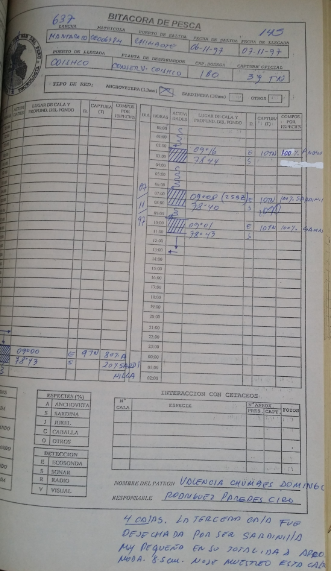
\includegraphics[width=0.8\linewidth]{imagen_Manual_PBP/antig}
\caption{Modelo bitacoras del año 1997.}
\label{fig:inter}
\end{figure}
\begin{figure}
\centering
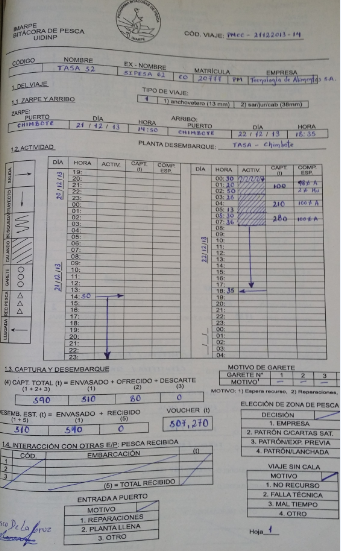
\includegraphics[width=0.8\linewidth]{imagen_Manual_PBP/nueva}
\caption{Modelo bitacoras del año 2013}
\label{fig:inter}
\end{figure}

\begin{figure}
\centering
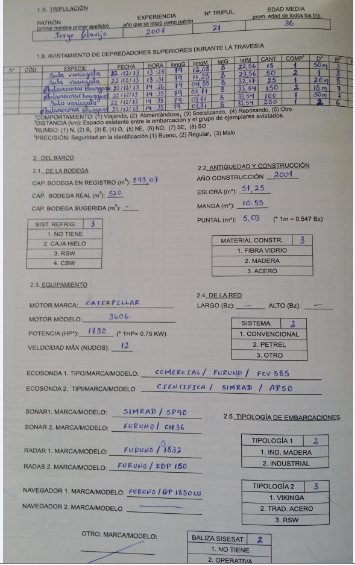
\includegraphics[width=0.8\linewidth]{imagen_Manual_PBP/nueva1}
\caption{Ejemplo datos avistamiento año 2013}
\label{fig:inter}
\end{figure}
 
 \begin{figure}
 \centering
 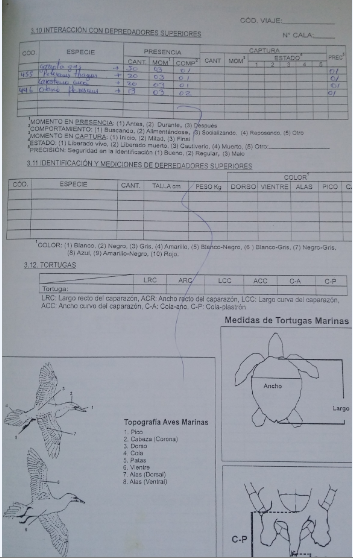
\includegraphics[width=0.8\linewidth]{imagen_Manual_PBP/nuevo2}
 \caption{Ejemplo datos interacción año 2013}
 \label{fig:inter}
 \end{figure}
 
\chapter{CONSIDERACIONES}
\section{Errores frecuente}
\begin{itemize}
\item{} Tipo de medición especies.
\item{} Duración según tipo de actividad.
\item{} Frecuencias de tallas elevadas para anchoveta.
\item{} Plantas distinta al lugar de desembarque.
\item{} Coordenadas fuera del límite.
\end{itemize}

\section{Casos especieales}
\begin{itemize}
\item{} Temperatuas bajas.
\item{} Bitacoreros repetidos en viajes distintos pero de la misma fecha.
\item{} Capturas elevadas a la capacidad de bodega embarcación.
\item{} Viajes incompletos.
\end{itemize}

\section{Recomendaciones}
\begin{itemize}
\item{} Registrar aquella observaciones que no se pudieran ingresar en cualquier otro item, de manera concreta, en las observaciones generales o referentes a las calas.
\item{} Comprobar la coencidencia entre la captura total y por calas.
\item{} Leer y registrar adecuadamente todos los datos existentes en las bitácoras de pesca.
\item{} Evitar hacer $"$check$"$ en viajes que no sean su objetivo.
\end{itemize}
\section{Glosario de términos}
\begin{itemize}
\item{\textbf{Sistema CSW:}} sistema de refrigeración mediante el cual se emplea agua de mar y hielo.

\item{\textbf{Gareta :}} cable acerado que jala la red de cerco  por intermedio del winche  durante la faena de pesca y que es acomodado en los carretes para su posterior lance. 

\item {\textbf{Carrete:}} cilindro generalmente con el eje hueco con bordes de discos en sus bases en que se enrollan los cables 

\item {\textbf{Loberíos:}} lugar o aposento de los lobos marinos (islas, penínsulas o playas).

\item{\textbf{Lobada:}} gran grupo de Lobos marinos buscando alimentos o acompañando a las embarcaciones pesqueras durante la faena de pesca.

\item{\textbf{Winche:}}  equipo de tambores giratorios hidráulicos de gran fuerza que facilitan la maniobra de pesca  al estibar la red o cualquier actividad en la cubierta de la embarcación el cual pueden ser de fricción o de combinación. 
  
\item{\textbf{Blancor:}} término pesquero al momento de visualizar superficialmente cardúmenes de color plateado a poca distancia.

\item{\textbf{Morado:}} término pesquero en visualizar superficialmente cardúmenes de color negro o morado en alta mar, mayormente se menciona en la pesca de anchoveta y sardina.
  
\item{\textbf{Macaco:}} cilindro metálico reforzado con caucho  ubicada en la parte  superior de la pluma que facilita la maniobra de jala gran parte de la red de cerco  para estibar ha cubierta en la popa de la embarcación.   

\item{\textbf{Net winch:}} cilindro hueco metálico reforzado con caucho, ubicado generalmente al lado estribor popa cuya función es facilitar  la operatividad de jalado de la red de cerco durante la actividad pesquera o lavado  de red desde el mar a cubierta el cual es parte de un moderno sistema de estibación de la red de cerco.

\item{\textbf{Net Staker:}} brazo hidráulico  metálico con un rodillo reforzado con caucho ubicado en la parte superior  que facilita la acomodación  de la red de cerco en popa y que es parte de un moderno sistema de estibación de la red de cerco.

\item{\textbf{Sistema RSW:}} sistema Conocido como ( Refrigerated Sea Water ) es decir refrigerado con agua de mar que consiste básicamente en almacenar la captura en bodega  con agua refrigerada circulando a +- $0^{\circ}$C lo que permite enfriar grandes cantidades a granel desde su captura hasta su desembarque. 

\item{\textbf{Ronza:}} denominación de la actividad del barco en alta mar, cuando esta al garete esperando recurso.

\item{\textbf{Pajarada:}} gran grupo de aves marinas en alta mar o en islas.
  
\item{\textbf{Proa:}} terminología naval que identifica la parte delantera de un barco, con la cual corta las aguas.

\item{\textbf{Popa:}} terminología naval que identifica la parte trasera  de un barco.
 
\item{\textbf{Babor:}} terminología naval que identifica el lado izquierdo de un barco.

\item{\textbf{Estribor:}} terminología naval que identifica el lado derecho de un barco.

\item{\textbf{Panga:}} embarcación Auxiliar ubicada en popa de la embarcación o bolichera cuya función es apoyar a jalar la red en el mar en  el proceso de cercado de la bolichera a un cardumen detectado durante toda la faena pesquera, a su vez permite apoyar  la estabilidad de la bolichera para evitar  enredo de red con la hélice o durante la estibación a cubierta de la red.

\item{\textbf{Chanchada:}} terminología pesquera  a un grupo de marineros marinos generalmente delfines.

\item{\textbf{Pericas:}} denominación pesquera a un grupo de gaviotas dominicanas.
 
\item{\textbf{Cochos:}} denominación a un grupo de pelicanos durante la faena de pesca.

\item{\textbf{Corte:}} se menciona al proceso de separar la red en el mar en dos partes mediante un cable, cuando el patrón de pesca considera que es una buena captura, facilitando estibar   la red y embazar la pesca con mayor facilidad evitando desestabilizar a la embarcación, posibles hundimientos  o accidentes durante la faena de pesca. 

\item{\textbf{Loberíos:}} lugar de reproducción o aposentos de  los lobos marinos ( islas, penínsulas o playas ).

\item  {\textbf{Secado:}}  es cuando queda poca pesca en la red de cerco al finalizar  la operatividad del absorbente para luego culminar  con la estiba de la red a cubierta.

\item {\textbf{Cabecero:}} cabo con el cual se sujeta el puño en el arte de cerco.

\item{\textbf{Ralo:}} se define como poca pesca  o  cuando el recurso está muy disperso para pescar. 

\end{itemize}

\chapter{REFERENCIAS}
\begin{enumerate}
\item Bouchon M., Ñique M., Arias M. y Bello R. 1998. Manual de Operaciones del Proyecto de Bitácoras de Pesca. Informe Progresivo Nro. 74. Instituto del Mar de Perú.
\item Carbajal Villalta W. 2009. Zonificación de la biodiversidad en el litoral de Piura. Instituto del Mar de Perú, sede regional de Piura. Recuperado de: \url{http://www.imarpe.gob.pe/paita/conferencias/zee_marino_costero.pdf} 
\item Chirichigno, N. Clave para identicar los peces marinos del Perú. Seguna Edición. Instituto del Mar Perú. 1998.
\item Tallas Mínimas y Porcentaje de Tolerancia Máxima de Juveniles de Recursos Hidrobiológicos. Instituto del Mar de Perú. Recuperado el 20 de mayo del 2015 de:\url{http://www.imarpe.pe/imarpe/tallas_minimas/tallas_minimas.php}


\end{enumerate}





\mainmatter  




\label{ch:capituloB} 
% ... (contenido del cap�tulo B)

%\appendix % Ap�ndices 
%\chapter{Apéndice X} 
%\label{ch:apendiceX} 


%\tableofcontents  Tabla de contenido 
 
\listoffigures  Índice de figuras 
 
%\listoftables  Índice de tablas 
%\newpage 



%\backmatter 
% Bibliograf�a 
%\include{bibliografia}

\end{document}